
\documentclass[10pt, conference, compsocconf]{IEEEtran}

% Packages
\usepackage[pdftex]{graphicx}

% for tables (use if required!)
\usepackage{setspace}
\usepackage{longtable}
\usepackage{colortbl}
\usepackage{array}
\usepackage{ragged2e}
\usepackage{lscape}
\usepackage{tabularx}
\usepackage{multirow}
\usepackage{booktabs}
\usepackage{url} 

%Anpassung der Namen f\"ur Abbildung und Tabelle
\usepackage[figurename={Abbildung},tablename={Tabelle}]{caption}

% Better handling of floats
\usepackage{float}

\newcolumntype{w}[1]{>{\raggedleft\hspace{0pt}}p{#1}}
\newcolumntype{x}[1]{>{\centering\hspace{0pt}}p{#1}}


% Set spaces between and after floats here:
\setlength{\textfloatsep}{8pt} % Vertical space below (above) [t] ([b]) floats


\newcommand{\conforms}{\mathrel{\widehat{=}}}


% correct bad hyphenation here
\hyphenation{}


% correct bad hyphenation here
\hyphenation{op-tical net-works semi-conduc-tor}


\begin{document}
\title{Entwicklung einer Einkaufslisten-App}


\author{\IEEEauthorblockN{Markus H\"ul\ss}
\IEEEauthorblockA{
E-Mail: huma1200@stud.hs-coburg.de}
\\
\IEEEauthorblockN{Tanja M\"ogn}
\IEEEauthorblockA{
E-Mail: mota1200@stud.hs-coburg.de}
\and
\IEEEauthorblockN{Malcolm K\"ogler}
\IEEEauthorblockA{
E-Mail: koma1200@stud.hs-coburg.de}
\\
\IEEEauthorblockN{Daniel M\"uller}
\IEEEauthorblockA{
E-Mail: muda1200@stud.hs-coburg.de}
}

% make the title area
\maketitle


\begin{abstract}
Mangels Verf\"ugbarkeit von multiplattformf\"ahigen Apps zur Verwaltung von Einkaufslisten entstand die Idee, eine solche App zu entwickeln. Um den Entwicklungsaufwand m\"oglichst gering zu halten und nicht f\"ur jede Plattform separat eine App programmieren zu müssen, entschieden wir uns f\"ur das Framework Phonegap. Dieses Paper besch\"aftigt sich mit der Konzeption und Entwicklung der App.   
\end{abstract}

\IEEEpeerreviewmaketitle

\section{Einleitung}
% no \IEEEPARstart
Immer pr\"asent und nicht mehr aus dem Alltag wegzudenken, unterst\"utzt  uns das Smartphone schon heute bei der Organisation und Kommunikation. 
Vor einigen Jahren musste vor dem Einkauf noch schnell ein Einkaufszettel geschrieben werden. 
Aber wie schnell war der Zettel  in der Tasche spurlos verschwunden. 
Da das Smartphone praktisch immer bei einem ist, bietet es sich als M\"oglichkeit an, einen Einkaufszettel zu speichern. 
Das schafft den Vorteil den Einkaufszettel jeder Zeit zu editieren oder ihn mit Freunden zu teilen. 
Ziel dieser Arbeit ist es, eine App zur Verwaltung von Einkaufszetteln zu entwickeln.
Diese soll es erm\"oglichen, erstellte Einkaufszettel mit anderen zu teilen.
Die jeweilige Plattform des App-Benutzers darf dabei kein Hindernis sein.

Die Projektgruppe wurde in zwei Teams aufgeteilt. 
Ein Team war f\"ur die Frontend-Entwicklung zust\"andig, das andere f\"ur das Backend. 
Der Programmcode wurde mittels des Versionierungssystems GIT verwaltet. 
Grafiken wurden mit Balsamiq und MS Visio 2013 erstellt. 
Die Kommunikation erfolgte teils pers\"onlich, teils \"uber E-Mails.

Zu Beginn wird die Konkurrenzanalyse beschrieben. 
Anschließend wird die Notwendigkeit von Mockups erläutert. 
Darauf folgend werden die verwendeten Technologien in Frontend und Backend vorgestellt. 
Zuletzt werden in einer Zusammenfassung die Projekterfolge und Misserfolge aufgezeigt.
Ein Ausblick zeigt die weiteren geplanten Entwicklungsschritte.

\section{Konkurrenzanalyse}
Um sich einen \"Uberblick \"uber vorhandene Apps zu verschaffen, wurde eine Konkurrenzanalyse erstellt.
Diese Konkurrenzanalyse beschr\"ankt sich auf native Apps und l\"asst Cloud-basierte L\"osungen au{\ss}en vor.
Zu diesem Zweck wurden die Top-Apps aus den App-Stores f\"ur die Plattformen Android, IOS und Windows Phone miteinander verglichen.
Der Vergleich erfolgte anhand der Kriterien Plattformunabh\"angigkeit bzw. Multiplattformf\"ahigkeit, Multiuserf\"ahigkeit der Einkaufslisten, sowie eine zentrale Datenhaltung mit Sychronisierung der Daten.

Am Markt gibt es mehrere Apps, die eine Alternative zum Papiereinkaufszettel darstellen.
Bez\"uglich der Plattformunabh\"angigkeit wurde festgestellt, dass es derzeit nur eine App gibt, die eine native Implementierung f\"ur die oben genannten Plattformen bereitstellt. 
Andere L\"osungen bieten eine reduzierte Multiplattformf\"ahigkeit in dem Sinne, dass ein Webservice zu Verf\"ugung gestellt wird.
\"Über diesen kann auf die Daten zugegriffen werden.
Die zentrale Datenhaltung wird bei den meisten Apps durch ein Backbone gel\"ost.
Multiuserf\"ahigkeit wird von wenigen Apps implementiert. Diese ist teilweise darauf beschr\"ankt, dass eine Einkaufsliste per E-Mail verschickt wird.

\section{Mockups}
Damit jedes Teammitglied eine Vorstellung davon hat, wie die App sp\"ater aussehen soll, war ein Prototyp notwendig.
Zu diesem Zweck wurden Mockups f\"ur das Frontend in Teamarbeit entworfen. 

\begin{figure}[h!]
	\centering
	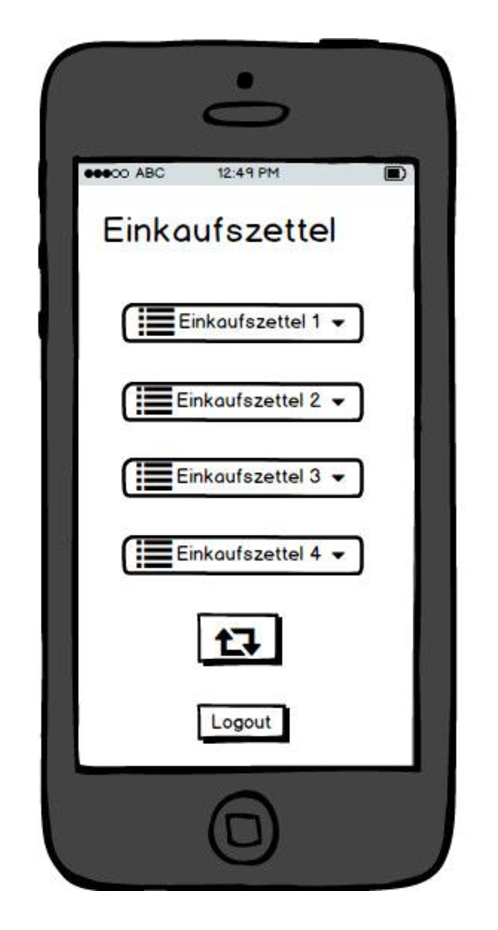
\includegraphics[scale=0.3]{./Bilder_Zeichnungen/Uebersicht.pdf}
	\caption{Einzelansicht}
	\label{fig:Mockup_Einzelansicht}
\end{figure}
In Abbildung~\ref{fig:Mockup_Einzelansicht} ist ein Beispiel f\"ur ein Mockup zu sehen. Die Abbildung~\ref{fig:Mockup_Einzelansicht} zeigt die Ansicht eines Einkaufszettels mit den zugeh\"origen Steuerelementen.

\section{Frontend}
Ein wichtiges Ziel ist es, eine plattform- und aufl\"osungsunabh\"angige Darstellung zu erm\"oglichen. 
Dabei soll das Frontend nicht f\"ur jede Plattform separat entwickelt werden.
Dies soll sowohl den Zeitaufwand als auch potenzielle Fehlerquellen verringern. 
Der Browser dient als Grundlage f\"ur die Darstellung. 
Somit ist eine Darstellung auf mobilen Ger\"aten und Desktop-PCs m\"oglich.
Dieser Abschnitt befasst sich mit den beiden Komponenten "Phonegap" und "jQuery mobile".

\subsection{Phonegap}
Die auf dem Markt vorhandenen Applikationen entwickeln f\"ur die Plattformen Android, iPhone und Windows Phone jeweils se\-parate native Apps. 
Das erfordert tiefgehendes Know-how f\"ur die einzelnen Plattformen. Zudem wird die Behandlung von Fehler- und Change-Requests aufw\"andig, da diese f\"ur jedes System separat entwickelt werden m\"ussen. 
Aus diesem Grund wird bei der Entwicklung der App auf Phonegap gesetzt. Phonegap ist ein Framework zum Erstellen von nativen Anwendungen f\"ur die g\"angigsten mobilen Plattformen durch die Verwendung von HTML5.
Das Konzept von Phonegap ist, zum einen das Frontend der Anwendung \"uber eine angezeigte Webseite im Browser zu realiseren. 
Zum anderen stellt es zus\"atzlich Javasript API's bereit, die einem Zugriff auf bestimmte Hardware eines Smartphones, wie beispielsweise Kamera oder Sensoren erm\"oglichen. 
Wichtig ist, dass man damit auf plattformabh\"angige Events reagieren kann, zum Beispiel auf eine schwache Funkverbindung des Ger\"ats. 
Somit sind Funktionalit\"aten nativer Apps gegeben, ohne sich intensiv mit der Architektur der Zielplattformen zu besch\"aftigen.
Der Buildprozess von Phonegap erstellt aus den Komponenten eine native App, welche sich zugeh\"origen App Store verkaufen l\"asst.

\subsection{jQuery Mobile}
Ein weiters Problem ist, dass sich die App nicht durch die Vielzahl an unterschiedlichen Browsern und Displayaufl\"osungen der Endger\"ate beinflussen l\"asst. 
Die Anwendung soll ein einheitliches Design, unabh\"angig von Browser und Aufl\"osung darstellen. 
Der Nutzer der Anwendung muss auf allen Browsern, mobil und Desktop, das gleiche Design sehen.
Um diese Anforderung zu erf\"ullen, wird auf das jQuery Mobile Framework zur\"uckgegriffen.
Es erm\"oglicht eine einfache Umsetzung von Webseiten mit einem responsive Design. Dieses Frameworkt wird von einer gro{\ss}en Anzahl an unterschiedlichen Browsern unterst\"utzt (sowohl mobile als auch non-mobile). 
Somit wird mit einer einzigen Version des Frontends eine gro{\ss}e Menge an Endger\"aten unterst\"utzt. Dies tr\"agt zu einer schnellen Entwicklung der Anwendung bei. 
Des weiteren ist es mit dem Multi-Page-Layout-Konzept m\"oglich, mit einer einzigen HTML-Seite alle Ansichten einer App darzustellen. 
Dadurch muss nicht bei jedem Wechsel einer Ansicht eine neue Seite heruntergeladen werden. Damit verbessert sich die Performance und Traffic wird gespart. (Bisherige Quelle bisher nur die jQuery Mobile-Website)

\section{Backend}
Ein weiteres wichtiges Ziel ist es, eine endger\"ateunabh\"angige Datenspeicherung zu gew\"ahrleisten. 
Daf\"ur ist ein Backend, das von \"uberall \"uber das Internet zu erreichen ist, vonn\"oten. 
F\"ur die Umsetzung des Projekts entschieden wir uns f\"ur einen Webserver. Bei der Datenhaltung wird PHP und MySQL genutzt. 
Die Kommunikation zwischen Frontend  und Backend erfolgt über JSON nach dem REST-Paradigma .  
Dieser Abschnitt befasst sich mit den Komponenten PHP, MySQL und JSON.

\subsection{PHP}
PHP wird im Backend verwendet, um die Schnittstelle zwischen Anwendung und Datenbank auf dem Webserver zu stellen. PHP unterst\"utzt unz\"ahlige Datenbanktypen und bietet ein breites Spektrum an Funktionalit\"aten zur Konvertierung in das JSON-Format.

\subsection{MySQL}
MySQL ist ein weit verbreitetes relationales Datenbanksystem und kam vor allem wegen seiner Platt\-formunabh\"angigkeit und der kostenfreien Nutzung unter der OpenSource-Lizenz zur Umsetzung der Datenbank in Frage. 
Ein weiteres Kriterium, das für MySQL sprach, war die M\"oglichkeit damit verschiedene Speicherssubsystemen zu nutzen. 
Durch die Verwendung von InnoDB stehen Rollback und Transaktionssicherungsm\"oglichkeiten zur Verf\"ugung. 
Das ist ein wichtiger Gesichtspunkt im Bezug auf Datensicherheit.

\begin{figure*}[t]
	\centering
	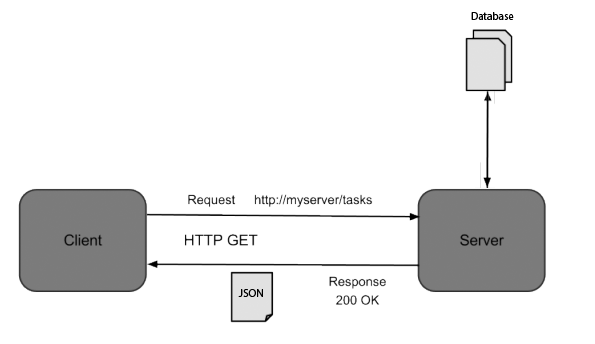
\includegraphics[width=0.8\textwidth]{./Bilder_Zeichnungen/Architektur_2.png}
	\caption{3-Wege-Architektur f\"ur die App}
	\label{fig:Architektur}
\end{figure*}

\subsection{JSON}
Aufgrund der Verwendung des auf Javascript basierenden Frameworks JQuery-Mobile, lag die Verwendung von JSON nahe.
Damit ist es können Daten vom Backend ohne spezielle Konvertierung in der Anwendung verwendet werden. 
Mithilfe von PHP l\"asst sich so die Schnittstelle nach dem REST-Programmierparadigma gestalten.

\section{Architektur}
{Damit die einzelnen Komponenten ordnungsgem\"a{\ss} zusammenarbeiten wird die passende Architektur ben\"otigt. Aufgrund der verwendeten Technologien wird eine Drei-Schichten-Architektur verwendet. Somit l\"asst sich eine Trennung von Pr\"asentation und Anwendungslogik realisieren.
	
Die Abbildung~\ref{fig:Architektur} zeigt den genauen Aufbau der Architektur. Ein Client sendet seine Aktion per HTTP-Request an den Webserver. Dieser holt die geforderten Daten aus der Datenbank oder \"andert diese. Die von der Datenbank erhaltenen Daten werden in das JSON-Format konvertiert. Danach werden sie als Inhalt des HTTP-Response an den Client gesendet. Der genauere Ablauf ist im Abbildung~\ref{fig:Sequenzdiagramm} ersichtlich.

\begin{figure}[h!]
	\centering
	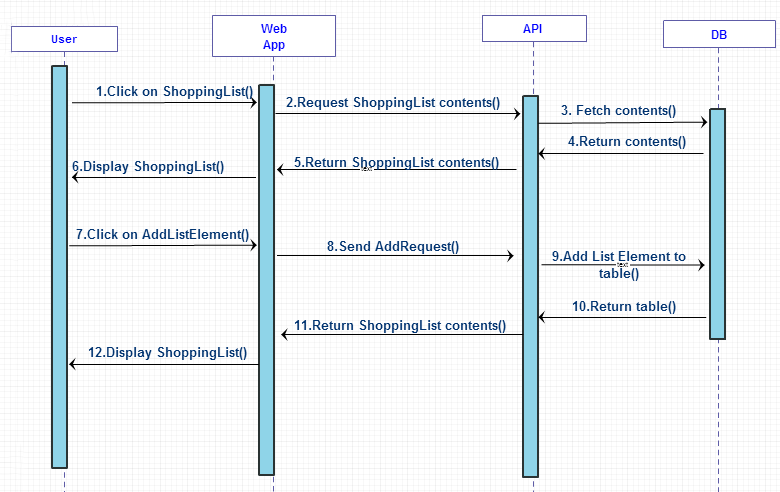
\includegraphics[width=0.45\textwidth]{./Bilder_Zeichnungen/Sequenzdiagramm.png}
	\caption{Sequenzdiagramm}
	\label{fig:Sequenzdiagramm}
\end{figure}

\section{Fazit}
Der Vorteil von Phonegap ist, dass ohne gro{\ss}e R\"ucksichtnahme auf die Plattform entwickelt werden konnte. 
Der Einsatz von JQuery mobile schafft eine einheitliche Darstellung der mobilen Web-App auf allen Ger\"aten.
Die Einbindung von anderen Frameworks ist mit Komplikationen verbunden.
Der Grund daf\"ur ist, dass viele Javascript-Frameworks den DOM-Tree manipulieren. 
Somit musste auf Frameworks wie AngularJS, welche eine Entwicklung nach dem MVC Pattern erm\"oglicht h\"atten, verzichtet werden.


\section {Ausblick}
Die App besitzt bereits alle notwendigen Funktionen, um eine Einkaufsliste zu erstellen, zu editieren und zu teilen. 
In der weiteren Entwicklung zeigen sich die Vorteile, die von Phonegap geboten werden. 
So kann beispielsweise ein Offline-Modus entwickelt werden, damit die App auch ohne permanente Internetverbindung nutzbar ist. 
%Das ist mit Phonegap m\"oglich, da man mit diesem Framework die Qualit\"at der Internetverbindung abfragen kann. 
Des Weiteren ist an eine intelligentere Unterst\"utzung der App im Alltag gedacht. 
Die App soll beispielsweise den User benachrichtigen, falls ein anderer User in einer gemeinsamen Einkaufsliste einen Eintrag ge\"andert oder hinzugef\"ugt hat. 
%Hier ist wichtig das unbedingt der native Benachrichtigungsmodus des Systems verwendet wird um so viel Usability wie m\"oglich zu %gew\"ahrleisten. 
Ein weitere Verbesserung w\"are auch die permanente Lokalisierung des Users und eine Reaktion der Einkaufslisten-App, wenn sich der User in der N\"ahe oder in einem Einkaufsladen befindet. 


\end{document}


